\tikzset{
	vdrwave/.pic={
			\path [pic actions, transform shape] plot [smooth, tension=1] coordinates {
			(0,0) (1,0.7) (2,0) (3,0.9) (4,0) (5,1) (6,0) (7,1) (8,0) (9,1) (10,0)
			(11,2.5) (12,0) (13,2.85) (14,0) (15,3) (16,0) (17,3) (18,0) (19,3) (20,0) 
			(21,1.5) (22,0) (23,1.2) (24,0) (25,1) (26,0) (27,1) (28,0)
			(29,1) (30,0)
		} ;
	},
	amplpic/.pic={
		\begin{scope}[xscale=0.06, yscale=.4]
			\pic [transform shape, draw=black!50] {vdrwave};
			\draw [ultra thick, <->] (6,0) to[ultra thick] (6,3);
		\end{scope}
	},
	pmoy/.pic={
		\begin{scope}[xscale=0.06, yscale=.4, ]
			\path [clip, transform shape] (-15,0) rectangle (22,3);
			\pic [transform shape, draw=black!50] {vdrwave};
			%\draw [ultra thick, <->] (6,0) to[ultra thick] (6,1);
			\draw (20,1.5) -- (6, 1.5) -- (0,2.2) node[left,
			font=\footnotesize] {$\overline{P_{i}}$};
			\draw (10,.5) -- (-2,.5) node[left, font=\footnotesize] {$\overline{P_{e}}$};
		\end{scope}
	}
}

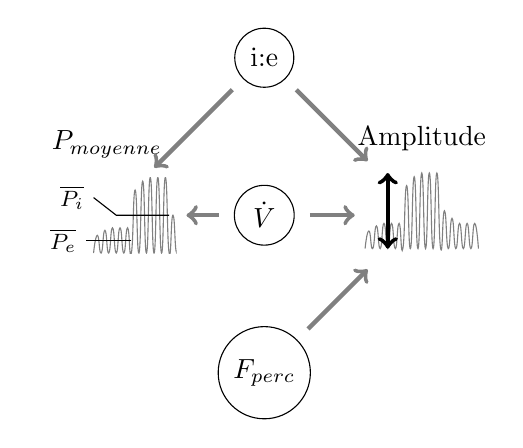
\begin{tikzpicture}	[
		node distance=2cm,
		link/.style={
			->,
			ultra thick,
			black!50,
		},
		indep/.style={
			draw,
			circle,
			outer sep=2mm,
			align=center,
		},
		target/.style={
			scale=0.8,
		},
	]

	\node [matrix,label=Amplitude] (A) {\pic [target] {amplpic};\\};
	\node [left of=A, indep] (D) {$\dot{V}$};
	\node [above of=D, indep] (R) {i:e};
	\node [below of=D, indep] (i) {$F_{perc}$};
	%\node [left of=D] (P) {$P_{moy_{insp.}}$};
	\node [left of=D, matrix,label=$P_{moyenne}$] (P) {\pic
	[target] {pmoy};\\};

	\draw [link] (D) -> (A);
	\draw [link] (R) -> (A);
	\draw [link] (i) -> (A);
	\draw [link] (D) -> (P);
	\draw [link] (R) -> (P);

\end{tikzpicture}
